\paragraph{}
Dans cette partie nous allons présenter plus en détails l'architecture globale du projet d'application mobile de Neuflize OBC. Comme nous l'avons vu précédemment, ce projet est basé sur une architecture multicouches dont la structure est représentée dans sa globalité figure \ref{archiLog}. Nous allons maintenant décrire l'objectif et le foncitonnement de chacune des couches afin de comprendre le fonctionnement du projet.

\subsection{API Security Gateway}
	TODO : blabla sur la couche
	
\begin{figure}[H]
	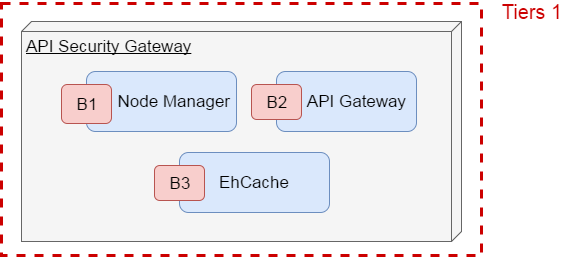
\includegraphics[scale=0.5]{images/travailNeuflizeOBC/architecture/coucheSecurity.png}
	\centering
	\caption{Couche API Security Gateway}
	\label{coucheSecurity}
\end{figure}

	\subsubsection{B1 - Node Manager}
	Gestion de la configuration logique (topologie, domaine, instance …), interagit avec la brique B18 (Admin Node manager) afin de permettre la scalabilité horizontale de la solution.
		
	\subsubsection{B2 - API Gateway}
	Serveur traitant les appels API. Cette brique est en charge de la sécurité applicative des appels vers la couche API Management. Positionnée dans le tiers 1, elle recevra les appels « HTTPS » et aura principalement pour objectif d’effectuer les actions suivantes : \\
	
	\begin{itemize}
		\item Terminaison TLS : vérification de la validité certificat partenaire
		\item Filtrage des requêtes 
		\item Firewall applicatif : vérification du contenu des messages REST
		\item Répartition de charge vers les composants en Aval
		\item Protection du SI : limitations du nombre d’appels API (mécanisme de régulation du traffic) et des appels au SI (mécanisme de cache)
		\item SLA (service Level Agreement) : collecte et trace des exécutions \\
	\end{itemize}
	
	\subsubsection{B3 - EhCache}
	Système de gestion de cache distribué en mémoire.
	
	\subsection{API Management}
	
	TODO : blabla sur la couche
	
\begin{figure}[H]
	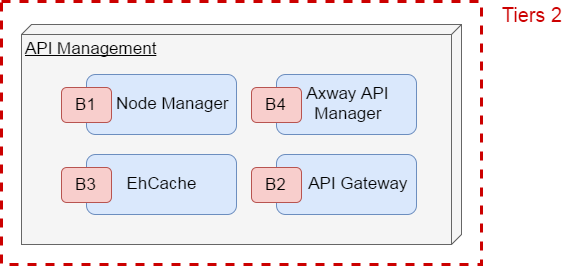
\includegraphics[scale=0.5]{images/travailNeuflizeOBC/architecture/coucheManagement.png}
	\centering
	\caption{Couche management}
	\label{coucheManagement}
\end{figure}

	\subsubsection{B4 - API Manager}
	Brique permettant de configurer et d’exposer des API. Elle contient également un mini serveur http pour proposer des pages statiques d’authentification utilisateurs. Elle assurera les fonctionnalités suivantes : \\
	
	\begin{itemize}
		\item Publication et sécurisation des API
		\item Gestion du cycle de vie des API
		\item Gestion de l’authentification et des habilitations (développeurs et administrateurs API)
		\item Embarquement des développeurs d’applications consommatrices d’API
		\item Audit, suivi de la consommation des API, gestions des quotas
		\item Haute disponibilité \\
	\end{itemize}

Deux instances d’API Gateway seront installées en mode « actif/actif ». La répartition de charge sera gérée par le composant API Gateway positionné en amont.
	
\subsection{Microservices}

	L'objectif de cette couche est de réaliser la composition des services métiers exposés par EFS dans le but d'exposer les données pour les applications ou les partenaires. L'architecture microservices est un paradigme d'architecture qui jouit actuellement d'une grande popularité aux dépends de celles plus classiques (N-tiers, SOA...), inventée afin de répondre aux problématiques soulevées par les projets de grande ampleur. \\
	
	Cette approche consiste à développer une application sous forme d'un ensemble de services dont la granularité correspond à une fonctionnalité élémentaire en terme métier. Chacun de ces services doit posséder son propre contexte d'exécution et ainsi être testable et déployable indépendemment en favorisant un couplage le plus faible possible. Ils peuvent être écrit dans des langages différents et communiquer entre eux via, par exemple, le protocole HTTP et la mise en place d'une API REST, ce qui est le cas pour ce projet. On parle alors de microservices, terme qui s'oppose aux applications plus classique que l'on dit monolithiques.\\
	
	Dans les gros projets, la quantité de code a tendance à augmenter rapidement impliquant une hausse de la compléxité et rendant ainsi difficile l'ajout de nouvelles fonctionnalités. Le couplage entre ces dernières devient fort et les nombreux effets de bords résultant de chaque modifications rendent alors l'application moins fiable, limitant les perspectives d'évolution. De plus, la scalabilité horizontale (par exemple un ajout de serveur) est elle aussi impactée. En effet, l'application entière doit être migrée si l'on souhaite changer de matériels afin d'améliorer les performances. Si un certain module est plus lent, il n'est pas possible de le déplacer indépendemment afin d'améliorer son exécution, il faut répliquer le monolithe entier.
	
	TODO : finir le blabla sur la couche
	
\begin{figure}[H]
	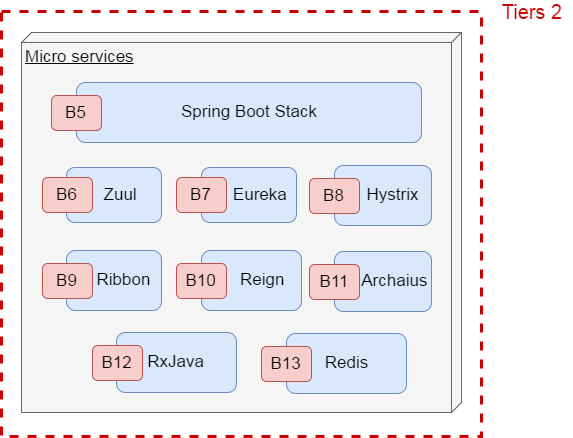
\includegraphics[scale=0.5]{images/travailNeuflizeOBC/architecture/coucheMicroservices.png}
	\centering
	\caption{Couche microservices}
	\label{coucheMicroservices}
\end{figure}

	\subsubsection{B5 - Spring Boot Stack}
	
Brique applicative hébergeant la couche micro service. C’est dans cette couche que de la composition de services pourra être réalisée (ex : services de l’API Backend EFS). Elle prendra en charge l’implémentation des principaux patterns d’implémentation de cette couche à savoir :
\begin{itemize}
	\item[Circuit breaker] : Capacité du système à être tolérant à la panne. En cas d’erreur successive lors de l’appel d’un sous-composant, le circuit d’appel est coupé « temporairement » en adoptant un comportement par défaut. 
	\item[Feature toggle] : Le principe est d’avoir une branche de développement et de déployer en production en continu. Ensuite l’activation d’une « feature » est pilotée par le business. Cela permet aussi d’activer une fonctionnalité en fonction d’une population ou une stratégie particulière. \\
\end{itemize}
	
	\subsubsection{B6 - Zuul}
	Gateway de l’architecture microservices fournissant des services de routage dynamique, surveillance, résilience et sécurité. Il sera notamment le point d’entrée unique de toutes les requêtes vers la couche micro service. L’implémentation choisie est Zuul de Netflix.
	
	\subsubsection{B7 - Eureka}
	Eureka est le serveur d’annuaire de services. Brique essentielle d'une architecture distribuée, le serveur d'annuaire permet la détection automatique des instances déployées. Les instances des applications sont accédées via leur nom plutôt que par leurs adresses physiques/IPs. Les applications n'ont plus besoin de connaitre les adresses des instances.
	
	\subsubsection{B8 - Hystrix}
	Hystrix est l'implémentation du pattern Circuit breaker permettant de contrôler la latence et les erreurs dues à des appels réseaux. L'idée essentielle est d'empêcher les erreurs en cascade dans un environnement distribué. Hystrix permet de 'fail-fast' mais de se rétablir rapidement créant ainsi une architecture tolérante aux erreurs capable de se rétablir de manière autonome (self-heal). Hystrix encapsule les appels extérieurs dans un thread à part permettant de configurer une méthode de fallback en cas d'erreur. Dès sa conception, le système prévoit les pannes.
De plus, Hystrix remonte des indicateurs concernant le résultat de la requête et le temps de réponse.

	\subsubsection{B9 - Ribbon}
	Librairie RPC gérant la communication inter-processus et qui fournit notamment des fonctionnalités de load-balancing côté client.
	
	\subsubsection{B10 - Reign}
	Librairie facilitant la création de service REST de façon déclarative.
	
	\subsubsection{B11 - Archaius}
	Archaius est le serveur de configuration. Il permet d’avoir une configuration centralisée pour les systèmes distribués. La configuration sera chargée directement depuis le repository de source GIT (brique B23).
	
	\subsubsection{B12 - RxJava}
	RxJava est une implémentation Java de Reactive Extensions : une bibliothèque permettant de créer des programmes asynchrones et événementiels en utilisant des séquences observables.
Il étend le modèle d'observateur pour prendre en charge les séquences de données / événements et ajoute des opérateurs qui permettent de composer des séquences de façon déclarative tout en s’abstrayant des problématiques telles que le bas-niveau threading, la synchronisation, la sécurité des threads et les structures de données concurrentes.
	
	\subsubsection{B13 - Redis}
	Redis cache manager blabla.

\subsection{Backend}

	TODO : blabla sur la couche
	
\begin{figure}[H]
	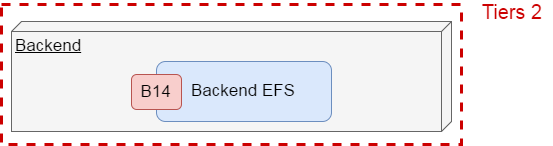
\includegraphics[scale=0.5]{images/travailNeuflizeOBC/architecture/coucheBackend.png}
	\centering
	\caption{Couche backend}
	\label{coucheBackend}
\end{figure}

	\subsubsection{B14 - EFS WeBank}
	Dans cette partie nous allons présenter plus en détails l'architecture globale du projet d'application mobile de Neuflize OBC. Comme nous l'avons dans la partie précédente, ce projet est basé sur une architecture multicouches dont la composition est représentée figure

\subsection{KPS Data}

	TODO : blabla sur la couche
	
\begin{figure}[H]
	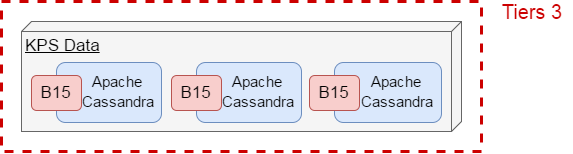
\includegraphics[scale=0.5]{images/travailNeuflizeOBC/architecture/coucheCassandra.png}
	\centering
	\caption{Couche KPS - Apache Cassandra}
	\label{coucheCassandra}
\end{figure}
	
	\subsubsection{B15 - Apache Cassandra}
	Apache Cassandra est un système de gestion de base de données (SGBD) de type NoSQL conçu pour gérer des quantités massives de données sur un grand nombre de serveurs, assurant une haute disponibilité en éliminant les points individuels de défaillance. Il permet une répartition robuste sur plusieurs centres de données3, avec une réplication asynchrone sans master et une faible latence pour les opérations de tous les clients. 
Apache Cassandra est requise pour stocker les données utilisées par le composant API Manager, par exemple le catalogue API, les quotas d’utilisation des API, les clients des API, etc… Cassandra peut être aussi utilisée pour le stockage des composants API Gateway suivants : \\

\begin{itemize}
	\item Key Property Store : table utilisé par API Gateway Server pour conserver des données utilisées lors de l’exécution des requêtes
	\item Magasin de jetons Oauth
	\item Répertoire Client : API Key et les données Oauth utilisées pour la sécurisation des API \\
\end{itemize}

\begin{figure}[H]
	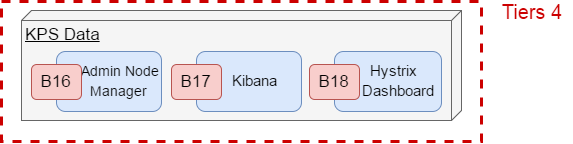
\includegraphics[scale=0.5]{images/travailNeuflizeOBC/architecture/coucheDashboard.png}
	\centering
	\caption{Couche KPS - Dashboards}
	\label{coucheDashboard}
\end{figure}
	
	\subsubsection{B16 - Admin Node Manager}
	C’est le serveur d’administration central d’un domaine API Gateway. Il permet notamment de réaliser toutes les opérations de déploiement, gestion de configurations dynamiques et surveillance de l’activité des instances API Gateway.
	
	\subsubsection{B17 - Kibana}
	Kibana est le module de Dashboard d'ElasticSearch. Il permet d'associer la puissance du moteur de recherche d'ElasticSearch (des recherches complexes peuvent être faites pour filtrer les données pertinentes à l'analyse) aux modules de reporting classiques.
	
	\subsubsection{B18 - Hystrix Dashboard}
	Permet d’effectuer du monitoring et de la gestion d’erreurs sur les services et applications grâce à un tableau de bord présentant les graphes et les métriques sur l’état des services de la plateforme.

\subsection{Monitoring}

	TODO : blabla sur la couche
	
\begin{figure}[H]
	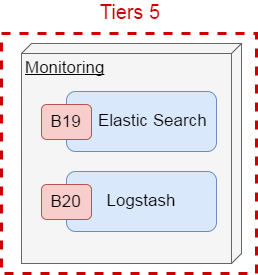
\includegraphics[scale=0.5]{images/travailNeuflizeOBC/architecture/coucheMonitoring.png}
	\centering
	\caption{Couche monitoring}
	\label{coucheMonitoring}
\end{figure}

	\subsubsection{B19 - ElasticSearch}
	Elasticsearch est un serveur utilisant Lucene (une bibliothèque open source écrite en Java qui permet d'indexer et de chercher du texte) pour l'indexation et la recherche des données. Il fournit un moteur de recherche distribué et multi-entité à travers une interface REST. C'est un logiciel libre écrit en Java et publié en open source sous licence Apache.
L'indexation des données s'effectue à partir d'une requête HTTP PUT. La recherche des données s'effectue avec la requête HTTP GET. Les données échangées sont au format JSON.
	
	\subsubsection{B20 - Logstash}
	Logstash est un outil pour collecter, traiter et transférer des événements et des messages de journal. La collecte s'effectue via des plugins d'entrée configurables, y compris la communication socket / paquet brute, le transfert de fichiers et plusieurs clients de bus de messages. Une fois qu'un plugin d'entrée a collecté des données, il peut être traité par un nombre quelconque de filtres qui modifient et annotent les données d'événement. Enfin Logstash envoie des événements aux plugins de sortie qui peuvent transmettre les événements à une variété de programmes externes y compris Elasticsearch, des fichiers locaux et plusieurs implémentations de bus de message.
	
\begin{figure}[h]
	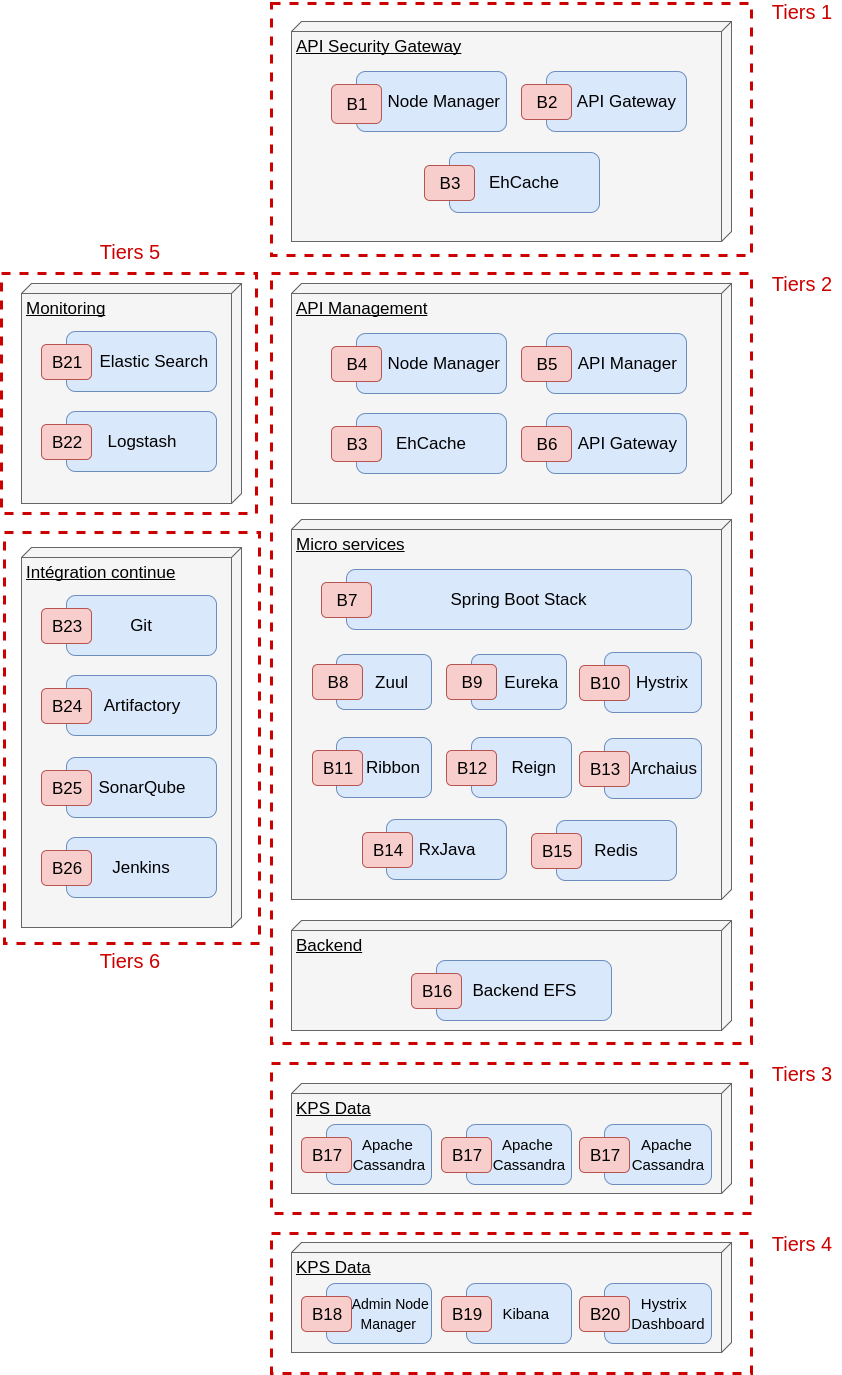
\includegraphics[scale=0.5]{images/travailNeuflizeOBC/architecture/architectureLogicielle.png}
	\centering
	\caption{Architecture logicielle}
	\label{archiLog}
\end{figure}

\newpage